In this section, the outcomes obtained from literature review conducted on the topic of Android application development are presented. Considering the tight relationship between the topic and industry, a Systematic Literature Review (SLR) was not adequate for finding relevant resources of data for the study. Hence, a Multivocal Literature Review (MLR) was conducted. As a type of SLR, MLR is collecting grey literature as well alongside formal literature \cite{40}. MLR considers resources like blogs, white papers, articles, academic literature and allows gathering information from academics, developers, practitioners, and independent researchers \cite{41}. Regardless of the direct relevance of the studies to maintainability, the research query presented in Fig. \ref{fig:lit_review_research_query} has been used to determine all the studies related to Android application development. For the purpose of obtaining more successful findings, the search query was separated into six parts, each of them individually focusing on a single topic.
\begin{figure}[ht!]
    \centering
    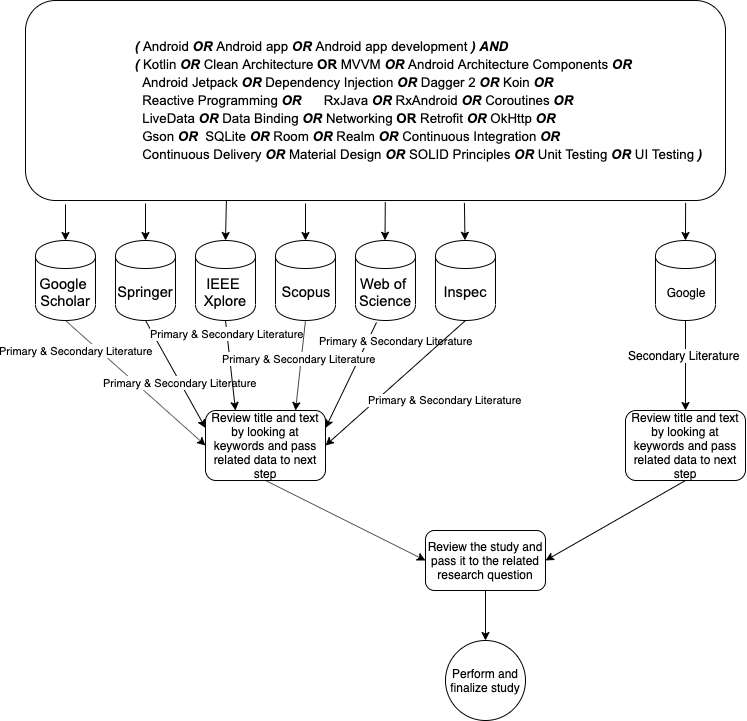
\includegraphics[scale=0.4]{figures/research_query.png}
    \caption{Search process visualization}
    \label{fig:lit_review_research_query}
\end{figure}
\FloatBarrier

After executing the query above, inclusion and exclusion criteria were applied to filter irrelevant studies. The inclusion and exclusion criteria are shown in Fig. \ref{fig:lit_review_research_query_criteria}.

\begin{figure}[ht!]
    \centering
    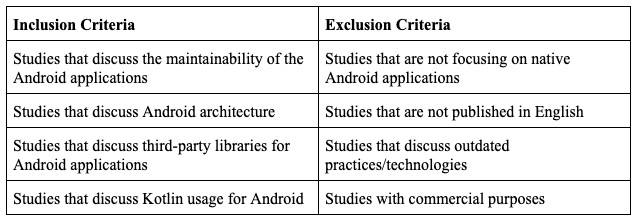
\includegraphics[scale=0.5]{figures/research_query_criteria.png}
    \caption{Inclusion and exclusion criteria}
    \label{fig:lit_review_research_query_criteria}
\end{figure}
\FloatBarrier

Finally, forty nine papers were found and reviewed. Grey literature results are not included in these numbers. However, the reviewed grey literature was also cited in this study.  The literature found as a result of this query was read thoroughly. Finally, inclusion and exclusion criteria were applied to the primary studies to have suitable literature only. As soon as the early research outcomes were collected, chasing the inclusion and exclusion criteria shown in Fig. \ref{fig:lit_review_research_query_criteria}, the unrelated material was filtered out. Also, the studies conducted before 2015 are excluded from the query results to prevent any possible up-to-dateness issues. Among the determined studies, those related to maintainability have been examined in more detail. These reviewed academic studies examined on Android application development can be grouped according to their topic titles as follows.
\begin{itemize}
    \item 4 studies bachelor theses regarding Android application development.
    \item 5 papers were related to 3rd party Android libraries.
    \item 6 papers were related to Kotlin programming language usage for Android.
    \item 6 papers were related to maintainability of the Android applications.
    \item 12 papers were related to Android app architecture.
    \item 16 papers were related to Android application development but not directly related to the topic that this study covers.
\end{itemize}

In addition to the papers mentioned above, 17 other papers are reviewed to get a better understanding of the studies conducted regarding software maintainability, metrics that can be used to measure software maintainability, general software engineering principles such as separation of concerns, and SOLID. These articles and books have been cited in various parts of this study.

Among the reviewed academic studies reviewed, the studies on Android application architecture and maintainability draw attention. Studies conducted on these two subjects account for more than one-third of the total studies examined. Based on these numbers, it can be said that the Android application architecture and the importance of maintainability are recognized by the researchers working in the Android field. In most of these studies, it is noteworthy that comparisons of Android application architectures in terms of performance, maintainability, and testability are common. As mentioned in previous chapters, considering the impact of software architecture on maintainability and the importance of maintainability in software development processes, it is not surprising that many academic studies have focused on these topics. Various studies on the maintainability of Android applications draw attention. For example, Hugo Källstrom (2016) conducted a study on a similar topic in which he implemented three different software architectures and evaluated the maintainability based on these architectures \cite{18}. Also, Prabowo et al. (2018) have a research on the maintainability of Android applications which they compared MVP and anti-pattern approaches \cite{19}. The research of Verdecchia et al. (2019) on architectural choices in Android applications is worth reading for both architecture and maintainability topics \cite{14}. Lastly, while the research of Saifan and Al-Rabad (2017) presents a different perspective on measuring the maintainability of Android applications \cite{34}, the study of Andrä et al. (2020) draws attention as the most recent research on this subject \cite{43}. On the other hand, most studies approach the maintainability of Android applications from an architectural perspective only. It is possible that other techniques and technologies can be used to increase the maintainability of Android applications besides architectural patterns. The fact that the studies do not focus on these techniques and technologies can be considered a limitation of the academic literature regarding this topic.